\documentclass[a4paper, 14pt]{extarticle}
\usepackage{float}
% Поля
%--------------------------------------
\usepackage{geometry}
\geometry{a4paper,tmargin=2cm,bmargin=2cm,lmargin=3cm,rmargin=1cm}
%--------------------------------------


%Russian-specific packages
%--------------------------------------
\usepackage[T2A]{fontenc}
\usepackage[utf8]{inputenc}
\usepackage[english, main=russian]{babel}
%--------------------------------------

\usepackage{textcomp}

% Красная строка
%--------------------------------------
\usepackage{indentfirst}
%--------------------------------------


%Graphics
%--------------------------------------
\usepackage{graphicx}
\graphicspath{ {./images/} }
\usepackage{wrapfig}
%--------------------------------------

% Полуторный интервал
%--------------------------------------
\linespread{1.3}
%--------------------------------------

%Выравнивание и переносы
%--------------------------------------
% Избавляемся от переполнений
\sloppy
% Запрещаем разрыв страницы после первой строки абзаца
\clubpenalty=10000
% Запрещаем разрыв страницы после последней строки абзаца
\widowpenalty=10000
%--------------------------------------

%Списки
\usepackage{enumitem}

%Подписи
\usepackage{caption}

%Гиперссылки
\usepackage{hyperref}

\hypersetup {
	unicode=true
}

%Рисунки
%--------------------------------------
\DeclareCaptionLabelSeparator*{emdash}{~--- }
\captionsetup[figure]{labelsep=emdash,font=onehalfspacing,position=bottom}
%--------------------------------------

\usepackage{tempora}

%Листинги
%--------------------------------------
\usepackage{listings}
\lstset{
  basicstyle=\ttfamily\footnotesize,
  %basicstyle=\footnotesize\AnkaCoder,        % the size of the fonts that are used for the code
  breakatwhitespace=false,        % sets if automatic breaks shoulbd only happen at whitespace
  breaklines=true,                 % sets automatic line breaking
  captionpos=t,                    % sets the caption-position to bottom
  inputencoding=utf8,
  frame=single,                    % adds a frame around the code
  keepspaces=true,                 % keeps spaces in text, useful for keeping indentation of code (possibly needs columns=flexible)
  keywordstyle=\bf,       % keyword style
  numbers=left,                    % where to put the line-numbers; possible values are (none, left, right)
  numbersep=5pt,                   % how far the line-numbers are from the code
  xleftmargin=25pt,
  xrightmargin=25pt,
  showspaces=false,                % show spaces everywhere adding particular underscores; it overrides 'showstringspaces'
  showstringspaces=false,          % underline spaces within strings only
  showtabs=false,                  % show tabs within strings adding particular underscores
  stepnumber=1,                    % the step between two line-numbers. If it's 1, each line will be numbered
  tabsize=2,                       % sets default tabsize to 8 spaces
  title=\lstname                   % show the filename of files included with \lstinputlisting; also try caption instead of title
}
%--------------------------------------

%%% Математические пакеты %%%
%--------------------------------------
\usepackage{amsthm,amsfonts,amsmath,amssymb,amscd}  % Математические дополнения от AMS
\usepackage{mathtools}                              % Добавляет окружение multlined
\usepackage[perpage]{footmisc}
%--------------------------------------

%--------------------------------------
%			НАЧАЛО ДОКУМЕНТА
%--------------------------------------

\begin{document}

%--------------------------------------
%			ТИТУЛЬНЫЙ ЛИСТ
%--------------------------------------
\begin{titlepage}
\thispagestyle{empty}
\newpage


%Шапка титульного листа
%--------------------------------------
\vspace*{-60pt}
\hspace{-65pt}
\begin{minipage}{0.3\textwidth}
\hspace*{-20pt}\centering

\includegraphics[width=\textwidth]{emblem}
\end{minipage}
\begin{minipage}{0.67\textwidth}\small \textbf{
\vspace*{-0.7ex}
\hspace*{-6pt}\centerline{Министерство науки и высшего образования Российской Федерации}
\vspace*{-0.7ex}
\centerline{Федеральное государственное бюджетное образовательное учреждение }
\vspace*{-0.7ex}
\centerline{высшего образования}
\vspace*{-0.7ex}
\centerline{<<Московский государственный технический университет}
\vspace*{-0.7ex}
\centerline{имени Н.Э. Баумана}
\vspace*{-0.7ex}
\centerline{(национальный исследовательский университет)>>}
\vspace*{-0.7ex}
\centerline{(МГТУ им. Н.Э. Баумана)}}
\end{minipage}
%--------------------------------------

%Полосы
%--------------------------------------
\vspace{-25pt}
\hspace{-35pt}\rule{\textwidth}{2.3pt}

\vspace*{-20.3pt}
\hspace{-35pt}\rule{\textwidth}{0.4pt}
%--------------------------------------

\vspace{1.5ex}
\hspace{-35pt} \noindent \small ФАКУЛЬТЕТ\hspace{80pt} <<Информатика и системы управления>>

\vspace*{-16pt}
\hspace{47pt}\rule{0.83\textwidth}{0.4pt}

\vspace{0.5ex}
\hspace{-35pt} \noindent \small КАФЕДРА\hspace{50pt} <<Теоретическая информатика и компьютерные технологии>>

\vspace*{-16pt}
\hspace{30pt}\rule{0.866\textwidth}{0.4pt}

\vspace{11em}

\begin{center}
\Large {\bf Лабораторная работа № 3 } \\
\large {\bf по курсу <<Численные методы линейной алгебры>>} \\
\large <<Реализация метода Гаусса c перестановками>>
\end{center}\normalsize

\vspace{8em}


\begin{flushright}
  {Студент группы ИУ9-71Б Баев Д.А \hspace*{15pt}\\
  \vspace{2ex}
  Преподаватель Посевин Д. П.\hspace*{15pt}}
\end{flushright}

\bigskip

\vfill


\begin{center}
\textsl{Москва 2023}
\end{center}
\end{titlepage}
%--------------------------------------
%		КОНЕЦ ТИТУЛЬНОГО ЛИСТА
%--------------------------------------

\renewcommand{\ttdefault}{pcr}

\setlength{\tabcolsep}{3pt}
\newpage
\setcounter{page}{2}

\section{Задание}\label{Sect::task}
1. Реализовать метод Гаусса с перестановками по столбцам, по строкам,
по столбцам и строкам одновременно для действительных квадратных
матриц произвольной размерности n.

2. Для проверки работоспособности алгоритмов необходимо использовать
алгоритм тестирования задачи написанный в лабораторной работе №2
«Реализация метода Гаусса».

3. Результат работы должен быть представлен в виде графиков зависимости
абсолютной погрешности вычислений классическим методом Гаусса,
методом Гаусса с перестановками по строкам, методом Гаусса с
перестановками по столбцам, методом Гаусса с перестановками по
столбцам и строкам, библиотечным методом от степени диагонального
преобладания. Все графики должны быть построены на одной
координатной плоскости. Напомним, что погрешность вычисления
вектора x системы линейных алгебраических уравнений A·x=b тем или
иным способом рассчитывается по Евклидовой норме разности точного
решения и решения полученного соответствующим методом. Степень
диагонального преобладания вычисляется, как максимальная разность по
i между модулем диагонального элемента и суммы модулей вне
диагональных элементов. Очевидно, что если значение степени
диагонального преобладания положительна, то условие диагонального
преобладания выполняется, в противном случае — не выполняется.
Поэтому график должен быть построен как для отрицательных значений
степени диагонального преобладания, так и для положительных.
\newpage
\section{Исходный код}

Исходный код программы представлен в листингах~\ref{lst:code1}--~\ref{lst:code4}.

\begin{figure}[H]
\begin{lstlisting}[language={},caption={Метод Гаусса c выбором главного элемента по столбцу},label={lst:code1}]
def gauss_column(A, b):
    n = len(A)
    A = deepcopy(A)
    b = deepcopy(b)

    for i in range(n - 1):
        max_index = np.argmax(np.abs(A[i:, i])) + i
        A[[i, max_index]] = A[[max_index , i]]
        b[i], b[max_index] = b[max_index], b[i]
        for j in range(i + 1, n):
            f = A[j][i] / A[i][i]
            A[j] -= f * A[i]
            b[j] -= f * b[i]

    x = np.zeros(shape=(n, ))

    for i in range(n - 1, -1, -1):
        x[i] = b[i] / A[i][i]
        for j in range(i - 1, -1, -1):
            b[j] -= A[j][i] * x[i]

    return np.array(x)
\end{lstlisting}
\end{figure}

\begin{figure}[H]
\begin{lstlisting}[language={},caption={Метод Гаусса с выбором главного элемента по строке},label={lst:code2}]
def gauss_row(A, b):
    n = len(A)
    A = deepcopy(A)
    b = deepcopy(b)
    x_i = [i for i in range(n)]

    for i in range(n - 1):
        max_index = np.argmax(np.abs(A[i, i:])) + i
        x_i[i], x_i[max_index] = x_i[max_index], x_i[i]
        for j in range(n):
            A[j][i], A[j][max_index] = A[j][max_index], A[j][i]
        for j in range(i + 1, n):
            f = A[j][i] / A[i][i]
            A[j] -= f * A[i]
            b[j] -= f * b[i]

    x = np.zeros(shape=(n, ))

    for i in range(n - 1, -1, -1):
        x[i] = b[i] / A[i][i]
        for j in range(i - 1, -1, -1):
            b[j] -= A[j][i] * x[i]

    x_copy = deepcopy(x)

    for i, order in enumerate(x_i):
        x[order] = x_copy[i]

    return np.array(x)
\end{lstlisting}
\end{figure}

\begin{figure}[H]
\begin{lstlisting}[language={},caption={Метод Гаусса с выбором главного элемента по столбцу и по строке},label={lst:code3}]
def gauss_row_and_column(A, b):
    n = len(A)
    A = deepcopy(A)
    b = deepcopy(b)
    x_i = [i for i in range(n)]

    for i in range(n - 1):
        max_index_col = np.argmax(np.abs(A[i:, i])) + i
        max_index_row = np.argmax(np.abs(A[i, i:])) + i
        if A[max_index_col][i] > A[i][max_index_row]:
            A[[i, max_index_col]] = A[[max_index_col , i]]
            b[i], b[max_index_col] = b[max_index_col], b[i]
        else:
            x_i[i], x_i[max_index_row] = x_i[max_index_row], x_i[i]
            for j in range(n):
                A[j][i], A[j][max_index_row] = A[j][max_index_row], A[j][i]

        for j in range(i + 1, n):
            f = A[j][i] / A[i][i]
            A[j] -= f * A[i]
            b[j] -= f * b[i]

    x = np.zeros(shape=(n, ))

    for i in range(n - 1, -1, -1):
        x[i] = b[i] / A[i][i]
        for j in range(i - 1, -1, -1):
            b[j] -= A[j][i] * x[i]

    x_copy = deepcopy(x)

    for i, order in enumerate(x_i):
        x[order] = x_copy[i]

    return np.array(x)
\end{lstlisting}
\end{figure}

\begin{figure}[H]
\begin{lstlisting}[language={},caption={Построение графика},label={lst:code4}]
dims = [10, 100, 300]
coofs = [i * 0.1 for i in range(1, 22, 3)]

for dim in dims:
    x = []
    y_classic = []
    y_rows = []
    y_columns = []
    y_both = []
    y_np = []
    for coof in coofs:
        A = generate_matrix(-10, 10, dim, diag=coof)
        x_vec = np.random.uniform(-10, 10, dim)
        x.append(get_diag_dom(A))
        y_classic.append(test_method(gauss, A=A, x=x_vec, debug=False))
        y_rows.append(test_method(gauss_row, A=A, x=x_vec, debug=False))
        y_columns.append(test_method(gauss_column, A=A, x=x_vec, debug=False))
        y_both.append(test_method(gauss_row_and_column, A=A, x=x_vec, debug=False))
        y_np.append(test_method(np.linalg.solve, A=A, x=x_vec, debug=False))
    plt.figure(figsize=(8, 4))
    plt.title(f'Dim: {dim}')
    plt.xlabel("diag_dom")
    plt.ylabel("Absolute error")
    plt.plot(x, y_classic, label='Classic')
    plt.plot(x, y_rows, label='Rows', color='red')
    plt.plot(x, y_columns, label='Columns', color='yellow')
    plt.plot(x, y_both, label='Both', color='green')
    plt.plot(x, y_np, label='Lib', color='black')
    plt.legend()
    plt.show()
\end{lstlisting}
\end{figure}

\section{Результаты}

Результат построения графика на матрице размерности 10x10 представлен на рисунке~\ref{fig:img1}.

\begin{figure}[H]
\centering
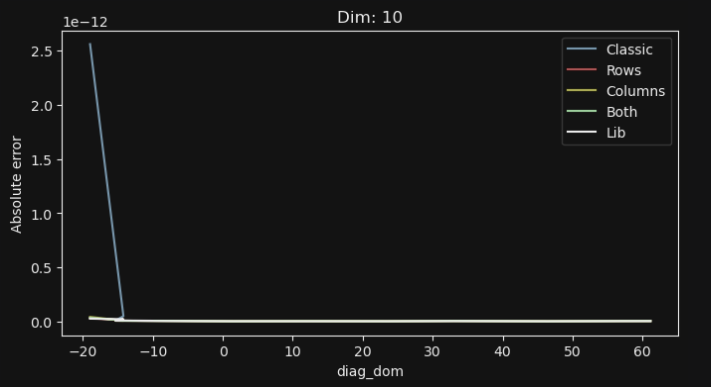
\includegraphics[width=0.8\textwidth]{images/res1.png}
\caption{Результат построения графика на матрице размерности 10x10}
\label{fig:img1}
\end{figure}


Результат построения графика на матрице размерности 100x100 представлен на рисунке~\ref{fig:img2}.


\begin{figure}[H]
\centering
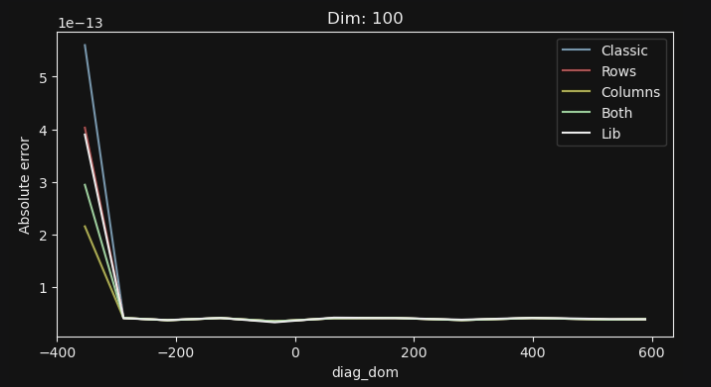
\includegraphics[width=0.8\textwidth]{images/res2.png}
\caption{Результат построения графика на матрице размерности 100x100}
\label{fig:img2}
\end{figure}


Результат построения графика на матрице размерности 300x300 представлен на рисунке~\ref{fig:img3}.

\begin{figure}[H]
\centering
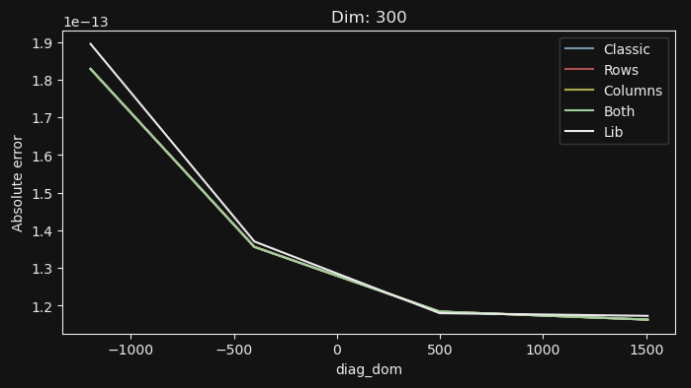
\includegraphics[width=0.8\textwidth]{images/res3.png}
\caption{Результат построения графика на матрице размерности 300x300}
\label{fig:img3}
\end{figure}


\section{Выводы}
В результате выполнения лабораторной работы были реализованы модификации метода Гаусса: с перестановками по столбцам, строкам или по столбцам и строкам одновременно.

Также была исследована зависимость абсолютной погрешности в результате работы классичесого метода Гаусса, его модификаций и библиотечного метода из Numpy от степени диагонального преобладания матрицы. Было обнаружено, что с появлением и ростом диагонального преобладания эти методы, особенно классический метод Гаусса, начинают выдавать все более точный ответ.
\end{document}